%!TEX root = ../main.tex

%\documentclass[twoside,twocolumn,a4j,dvipdfmx]{jarticle}
%\usepackage{amsmath,amssymb}
%\usepackage[dvipdfmx]{graphicx}
%\newcommand{\im}{\mathrm{i}}
%\newcommand{\bx}{\mathrm x}
%\newcommand{\R}{\mathbb{R}}
%\newcommand{\Largezero}{\mbox{\Large{0}}}
%\newcommand{\Hugezero}{\mbox{\Huge{0}}}
%\newtheorem{thm}{定理}[section]
%\newtheorem{df}[thm]{定義}
%\newtheorem{lem}{補助定理}[section]
%\newtheorem{prop}[thm]{補題}
%\setcounter{MaxMatrixCols}{100}

%\begin{document}
この章では、van der Pol方程式
$$
\frac{d^2 x}{dt^2} - \mu (1-x^2)\frac{dx}{dt} + x = 0
$$
の周期解の数値検証方法の詳細を記し、精度保証を行う。

\subsection{作用素$A^\dagger$ , $A$ の定義}

\subsubsection{$A^\dagger$ の定義}

Banach空間 $X= \mathbb{C} \times \ell^1_\nu, Y=\mathbb{C} \times \ell^1_{\nu'}$ ($\nu'<\nu$) と設定し、$A^\dagger$ を $A^\dagger \in \mathcal{L}(X,Y)$ として、$b=(b_0,b_1)\in \mathbb{C}\times \ell^1_\nu = X$に対して、 $A^\dagger b = ((A^\dagger b)_0 , (A^\dagger b)_1 )$ と作用するように定義する。ここで、 $A^\dagger$ を形式的に見ると、
\footnotesize
\begin{align*}
    A^\dagger &= 
    \left[\begin{array}{c|cccccc}
    0 & 1 &  \cdots  & 1 & \cdots & {0} & \cdots  \\\hline
    \vdots & &  \vdots & & & & \\
    \partial_\omega f_k & \cdots & \partial_{a_j} f_k & \cdots & & \Hugezero &\\
    \vdots& &  \vdots & & & & \\
    \vdots & & & & \lambda_N & & \Largezero   \\
    0 & & \Hugezero & & & \lambda_{N+1} & \\
    \vdots & & & & \Largezero& & \ddots
    \end{array}\right] \\
    &=
    \left[
    \begin{array}{c|c}
    0 & A_{a,0}^\dagger \\
    \hline 
    A_{\omega, 1}^\dagger & A_{a,1}^\dagger
    \end{array}
    \right].
\end{align*}
\normalsize
このことから、 $A^\dagger b$ は、
    \begin{align*}
    A^\dagger b &= 
    \begin{bmatrix}
    0 & A_{a,0}^\dagger \\
    A_{\omega ,1}^\dagger & A_{a,1}^\dagger
    \end{bmatrix}
    \times
    \begin{bmatrix}
    b_0 \\
    b_1
    \end{bmatrix} \\
    &=
    \begin{bmatrix}
    A^\dagger_{a,0} b_1 \\
    A^\dagger_{\omega ,1} b_0 + A^\dagger_{a,1} b_1
    \end{bmatrix}
    =: 
    \begin{bmatrix}
    (A^\dagger b)_0 \\
    (A^\dagger b)_1
    \end{bmatrix}
    \end{align*}
と表すことができ、
$$
    (A^\dagger b)_0 = \sum_{|k|<N} (b_1)_k
$$
\footnotesize
\begin{align*}
    ((A^\dagger b)_1 )_k &:= 
    \begin{cases}
    \partial_\omega f_k b_0 + \sum_{|j|<N} \partial_{a_j} f_k (b_1 )_j, &|k| < N  \\
    \lambda_k (b_1)_k &|k| \ge N
    \end{cases} \\
    \lambda_k &:= -k^2 \omega^2 - \mu \im k \omega + 1
\end{align*}
\normalsize
と具体的に書ける。またこのとき、$(A^\dagger b)_0$と$(A^\dagger b)_1$はそれぞれ
    \begin{align*}
    (A^\dagger b)_0 = A^\dagger_{a,0} b_1 = \sum_{|k|<N} (b_1)_k \in \mathbb{C} \\
    (A^\dagger b)_1 = A^\dagger_{\omega, 1} b_0 + A^\dagger_{a,1} b_1 \in \ell^1_{\nu^\prime}.
    \end{align*}

\begin{rem}
上のtail部分は実際には添字$k$に対して正負両方の向きに伸びているが、今回は一方向のみ表記している。
\end{rem}

\subsubsection{$A$ の定義}

次に作用素 $A$ について考える。 
$$
    A^{(N)} = 
    \begin{bmatrix}
    A_{\omega,0}^{(N)} & A_{a,0}^{(N)} \\
    A_{\omega,1}^{N)} & A_{a,1}^{(N)}
    \end{bmatrix}
    \approx DF^{(N)}(\bar{\bx})^{-1} \in \mathbb{C}^{2N \times 2N}
$$
をJacobi行列の近似逆行列とする。そして、$A \in \mathcal{L}(Y,X)$ として、$b = (b_0, b_1 ) \in X$に対して、 $Ab = ((Ab)_0, (Ab)_1)$ と作用するように定義する。ここで、
    \begin{align*}
    (Ab)_0 &= A_{\omega,0}^{(N)}b_0 + A_{a,0}^{(N)}b_1^{(N)} \\
    (Ab)_1 &= A_{\omega,1}^{(N)}b_0 + A_{a,1}b_1.
    \end{align*}
ただし、無限次元の $A_{a,1}b_1$ は以下のようになる。
$$
    (A_{a,1} b_1 )_k = 
    \begin{cases}
    (A_{a,1}^{(N)}b_1^{(N)})_k &(|k| < N) \\
    (b_1)_k / \lambda_k &(|k| \ge N).
    \end{cases}
$$
この定義を形式的に見ると
\begin{align*}
    A &=
    \left[
    \begin{array}{c|cccc}
    A^{(N)}_{\omega , 0} & A^{(N)}_{a,0} & 0 & \cdots & 0 \\
    \hline
    A^{(N)}_{\omega ,1} & A^{(N)}_{a,1} &  & \Largezero &\\
    0 & &\frac1{\lambda_{N}} &  & \\
    \vdots & & & \frac1{\lambda_{N+1}} & \\
    0 & & \Largezero & & \ddots
    \end{array}
    \right]\\
    &=
    \left[
    \begin{array}{c|c}
    0 & A_{a,0} \\
    \hline 
    A_{\omega, 1} & A_{a,1}
    \end{array}
    \right].
\end{align*}
と表記できる。

\subsection{$Y_0, Z_0, Z_1, Z_2$ の評価}

\subsubsection{$Y_0$の評価}
今、
$$
    F(\bar \bx) = (\delta_0 , \delta_1) \in \mathbb{C} \times \ell^1_{\nu'}
$$
とすると、$A$の定義より、
\begin{align*}
    \|AF(\bar \bx)\|_X \leq \max&\Biggl\{|A^{(N)}_{\omega, 0} \delta_0 + A^{(N)}_{a,0} \delta^{(N)}_1|,  \\
    &~ \left. \|A^{(N)}_{\omega,1} \delta_0 + A_{a,1} \delta^{(N)}_1 \|_{w} \right. \\
    &~ + \sum_{|k| > N} \left| \frac{(\delta^{\infty}_1)_k}{\lambda_k} \right| \nu^{|k|}\Biggr\}=:Y_0.
\end{align*}
ここで、$\delta_1=(\delta_1^{(N)}, \delta^{(\infty)}_1)\in\mathbb{C}^{2*3(N-1)+1}$であり、
$$
    (\delta_1)_k = 
    \begin{cases}
    \delta_1^{(N)} &(k < |N|) \\
    \delta_1^{(\infty)} &(k \geq |N|)
    \end{cases}
$$
と表した。

\subsubsection{$Z_0$の評価}
次に、 $Z_0$ の評価を与える。
$$
    % \begin{align*}
    B := I - AA^\dagger = \begin{bmatrix}
          B_{\omega , 0} & B_{a,0} \\
          B_{\omega, 1} & B_{a,1}
         \end{bmatrix}.
    % \end{align*}
$$
この $B$ を $c \in \overline{B(0,1)}, \| c \|_X \le 1$ である $c = (c_0, c_1)$ に作用させると、
    \begin{align*}
    (Bc)_0 &= B_{\omega,0} c_0 + B_{a,0}c_1 \\
    (Bc)_1 &= B_{\omega,1} c_0 + B_{a,1}c_1.
    \end{align*}
ここで、$(Bc)_0$ はスカラ値なので、
\begin{align*}
|B_{a,0} c_1| &\leq \sum_{k \in \mathbb{Z}}|(B_{a,0})_k||(c_1)_k| \\
&= \sum_{k \in \mathbb{Z}} \frac{|(B_{a,0})_k|}{w_k} |(c_1)_k|w_k \\
&\leq \underset{k < |N|}{\max} \frac{|(B_{a,0})_k|}{w_k} \sum_{k \in \mathbb{Z}} |(c_1)_k|w_k \\
&\leq \underset{k < |N|}{\max} \frac{|(B_{a,0})_k|}{w_k}, \\
&(\sum_{k \in \mathbb{Z} }|(c_1)_k|w_k = \|c_1 \|_w \le 1).
\end{align*}
よって、
$$
|(Bc)_0| \leq |B_{\omega,0}| + \underset{|k| < N}{\max} \frac{|(B_{a,0})_k|}{\omega_k} = Z_0^{(0)}.
$$
またここで、作用素 $M:\ell_{\nu}^1\to \ell_{\nu}^1$ の作用素ノルムについて以下の補題を準備する。

\begin{prop}
行列 $M^{(N)}$ を $M^{(N)} \in \mathbb{C}^{(2N-1) \times (2N-1)}$ 、双方向の複素無限点列(a bi-infinite sequence of complex numbers) を $\{ \delta_k \}_{|k| \geq N}$ と定義する。ここで、 $\delta_N > 0$ であり、
$$
    |\delta_k| \leq \delta_N \text{ for all } |k| \geq N.
$$
を満たすとする。そして、$a = (a_k)_{k \in \mathbb{Z}} \in \ell^1_\nu$ に対して 
$a^{(N)} = (a_{-N+1} , \dots, a_{N-1}) \in \mathbb{C}^{2N-1}$と表し、
作用素 $M:\ell_{\nu}^1\to \ell_{\nu}^1$ を以下のように定義する。
$$
    [Ma]_k := 
    \begin{cases}
    [M^{(N)}a^{(N)}]_k, & |k| < N \\
    \delta_k a_k ,& |k| \geq N.
    \end{cases}
$$
このとき、 $M$ は有界線形作用素であり、
\begin{align*}
    \|M\|_{\mathcal{L}(\ell^1_\nu)} &\leq \max{(K,\delta_N)},\\
    K &:= \max_{|n|<N} \frac{1}{\nu^{|n|}} \sum_{|k|<N} |M_{k,n}| \nu^{|k|}
\end{align*}
と評価される。
\end{prop}

上の補題を利用すると、
$$
    \| (Bc)_1 \|_w \leq \| B_{\omega,1} \|_w + \| B_{a,1} \|_{\mathcal{L}(\ell_\nu^{1})} = Z_0^{(1)}
$$
が評価可能となり、結論としては、求めたい $Z_0$ は $Z_0 := \{Z_0^{(0)}, Z_0^{(1)}\}$ となる。

\subsubsection{$Z_1$ の評価}
さらに $Z_1$ の評価を与える。 $Z_1$ は次の不等式を満たす。
\begin{align*}
    \|A(DF(\bar{\bx}) - A^\dagger ) c \|_X &\leq Z_1,\\
\mbox{ここで, }    c = (c_0, c_1) \in \overline{B(0,1)} \Leftrightarrow \|c \|_X &\leq 1.
\end{align*}
点列 $z$ を下記のように定義する。
$$
    z := (DF(\bar{\bx}) - A^\dagger ) c = 
    \begin{bmatrix}
    z_0 \\
    z_1
    \end{bmatrix}.
$$
ここで、$DF(\bar{\bx})$ と $A^\dagger$ は
$$
    DF(\bar{\bx}) =
    \left[\begin{array}{c|ccc}
    0 & \cdots & 1 & \cdots \\\hline
    \vdots & &\vdots&\\
    \partial_{\omega}f_k& \dots & \partial_{a_j}f_k & \dots\\
    \vdots & &\vdots& 
    \end{array}\right],
$$
\footnotesize
$$
    A^\dagger =
    \left[
    \begin{array}{c|cccccc}
    0 & \cdots & \partial_a \eta & \cdots & 0 & \cdots & 0 \\
    \hline
    \vdots &  & \vdots & & & & \\
    \partial_\omega f_{k}^{(N)} & \cdots & \partial_{a_j} f_{k}^{(N)} & \cdots & & & \\
    \vdots & & \vdots & & \Large{0} & \\
    0 & & & \lambda_{N} & & & \\
    \vdots & & & & \lambda_{N+1} & & \\
    0 & & \Large{0} & & & \ddots
    \end{array}
    \right],
$$
\normalsize
$$
    \lambda_k := -k^2 \omega^2 - \mu \im k \omega + 1
$$
と表される。すると $z_0$ は、
$$
    z_0 = \sum_{|k| \ge N} (c_1 )_k, |z_0| \leq \frac{1}{w_{N}} \sum_{|k| \ge N} |(c_1)_k| w_k \leq \frac{1}{w_{N}}.
$$

次に、 $z_1$ について考える。 $DF(\bar{\bx})c$ 部分は
    \begin{align*}
    ((DF(\bar{\bx})c)_1)_k &= \partial_\omega f_k c_0 + \partial_a f_k c_1 \\
    &= \frac{\partial \lambda_k}{\partial \omega} c_0 \bar{a}_k + \frac{\mu \im k}{3}(\bar{a} * \bar{a} * \bar{a})_k c_0 \\
    & ~+ \lambda_k (c_1)_k + \mu \im k \omega (\bar{a} * \bar{a} * c_1)_k, \\
    &\quad k \in \mathbb{Z}
    \end{align*}
と書け、 $|k| \geq N$ で $\bar{a}_k = 0$ より、 $c_1 = c_1^{(N)} + c_1^{(\infty)}$ として、

\footnotesize
$$
    (z_1)_k = 
    \begin{cases}
    \mu \im k \omega (\bar{a} * \bar{a} * c_1^{(\infty)})_k , ~ |k| < N\\
    \frac{\mu \im k}{3}(\bar{a} * \bar{a} * \bar{a})_k c_0 + \mu \im k \omega (\bar{a} * \bar{a} * c_1)_k, ~ |k| \geq N
    \end{cases}
$$
\normalsize
と表せる。ここから、 $z_1$ の絶対値をとると、 $|k| < N$ で
\begin{align*}
    |(z_1)_k| \leq |\mu \im k \omega| \max
    &\left\{ 
    \max_{k-N+1 \leq j \leq -N} \frac{|(\bar{a} * \bar{a})_{k-j}|}{w_j}, \right. \\
    &~~ \left. \max_{N \leq j \leq k+N-1} \frac{|(\bar{a} * \bar{a})_{k-j}|}{w_j}
    \right\} \\
    &=:\zeta,\quad \zeta = (\zeta_k)_{|k| < N} \in \mathbb{R}^{2N-1}.
\end{align*}

最後に、 $Z_1$ を求める。 $Z_1^{(0)}$ は次を満たすとする。
    \begin{align*}
    |(A(DF(\bar{\bx}) - A^\dagger)c)_0| &= |(Az)_0| \\
    &\leq |A_{\omega,0}^{(N)}| |z_0| + |A_{a,0}^{(N)}| | z_1^{(N)}| \\
    &\leq \frac{|A_{\omega,0}^{(N)}|}{w_{N}} + |A_{a,0}^{(N)}|\zeta \\
    &=: Z_1^{(0)}.
    \end{align*}
そして、$Z_1^{(1)}$ は次を満たすとする。
\footnotesize
    \begin{align*}
    \|(A(DF(\bar{\bx}) - A^\dagger)c)_1 \|_w &= \|(Az)_1 \|_w \\
    &= \| A_{\omega,1}^{(N)} z_0 + A_{a,1} z_1 \|_w \\
    &\leq \frac{\|A_{\omega,1}^{(N)} \|_w}{w_{N}} + \sum_{|k|<N} (|A_{a,1}^{(N)}| \zeta)_k w_k \\
    &~~+ \sum_{|k| \geq N} \frac{|\mu \im k (\bar{a}*\bar{a}*\bar{a})_k |}{3|\lambda_k |} w_k  \\
    &~~+ \sum_{|k| \geq N} \frac{ |\mu \im k \omega ( \bar{a} * \bar{a} * c_1 )_k |}{|\lambda_k|} w_k \\
    &\leq \frac{\|A_{\omega,1}^{(N)} \|_w}{w_{N}} + \sum_{|k|<N} (|A_{a,1}^{(N)}| \zeta)_k w_k\\
    &~~+ \sum_{N\le |k| \le 3(N-1)} \frac{|\mu \im k (\bar{a}*\bar{a}*\bar{a})_k |}{3|\lambda_k |} w_k  \\
    &~~+ \sum_{|k| \geq N} \frac{ |\mu \im k \omega ( \bar{a} * \bar{a} * c_1 )_k |}{|\lambda_k|} w_k \\
    &\leq \frac{\| A_{\omega,1}^{(N)} \|_w}{w_{N}} + \| |A_{a,1}^{(N)}| \zeta \|_w \\
    &~~+ \sum_{N\le |k| \le 3(N-1)} \frac{|\mu \im k (\bar{a}*\bar{a}*\bar{a})_k |}{3|\lambda_k |} w_k  \\
    &~~+ \frac{1}{N} \frac{\mu \omega \|\bar{a} \|_{w}^2}{\omega^2 - \frac{1}{N^2}} \\
    &=: Z_1^{(1)}.
    \end{align*}
\normalsize

よって、
$$
    Z_1 := \max\{Z_1^{(0)}, Z_1^{(1)}\}.
$$

\textbf{$Z_1^{(1)}$ の評価の補足}

上の評価に現れる
$$
\sum_{|k| \geq N} \frac{ |\mu \im k \omega ( \bar{a} * \bar{a} * c_1 )_k |}{|\lambda_k|} w_k \\
$$
は、$\lambda_k := -k^2 \omega^2 - \mu \im k \omega + 1$ より、次で評価される。
\footnotesize
\begin{align*}
\sum_{|k| \geq N} \frac{ |\mu \im k \omega ( \bar{a} * \bar{a} * c_1 )_k |}{|\lambda_k|} w_k 
&= \sum_{|k| \geq N} \frac{ |\mu \im k \omega ( \bar{a} * \bar{a} * c_1 )_k |}{|-k^2 \omega^2 - \mu \im k \omega + 1|} w_k \\
&\leq \sum_{|k| \geq N} \frac{1}{|k|} \frac{ |\mu \im \omega ( \bar{a} * \bar{a} * c_1 )_k |}{|\omega^2 + \frac{\mu \im \omega}{k} - \frac{1}{k^2}|} w_k \\
&\leq \sum_{|k| \geq N} \frac{1}{|k|} \frac{ |\mu \im \omega ( \bar{a} * \bar{a} * c_1 )_k |}{|\omega^2 - \frac{1}{k^2}|} w_k \\
&\leq \frac{1}{N} \frac{\mu \im \omega \|\bar{a} \|_{w}^2}{\omega^2 - \frac{1}{N^2}}.
\end{align*}
\normalsize

\subsubsection{$Z_2$ の評価}
最後に $Z_2$ の評価を与える。今、
$b \in \overline{B(\bar{\bx},r)}, c = (c_0, c_1) \in \overline{B(0,1)}$ について、 $Z_2$ の評価は次の不等式を満たす。
$$
    \| A(DF(b) - DF(\bar{\bx}))c \|_X \leq Z_2 (r)r
$$
まず $z$ を、
$$
    z := (DF(b) - DF(\bar{\bx}))c = 
    \begin{bmatrix}
    z_0 \\
    z_1 \\
    \end{bmatrix}
    =
    \begin{bmatrix}
    0 \\
    z_1 \\
    \end{bmatrix}
$$
と定義する。 $DF$ の定義から $z_0 = 0$ となるので、 $z_1$ だけを考えればよく、
\begin{align*}
    (z_1)_k := &(\partial_\omega f_k (b) - \partial_\omega f_k (\bar{\bx})) c_0 \\
     &+ [(\partial_a f(b) - \partial_a f(\bar{\bx}))c_1]_k , k \in \mathbb{Z}
\end{align*}
と書ける。$b = (\omega, (a_k)_{k \in \mathbb{Z}}), \bar{\bx} = (\bar{\omega}, (\bar{a}_k)_{|k| < N})$ として、第1項は、
    \begin{align*}
    &(\partial_\omega f_k (b) - \partial_\omega f_k (\bar{\bx}))c_0 \\
    &= \left[((- 2 k^2 \omega - \mu \im k)a_k + \frac{\mu \im k}{3} (a*a*a)_k) \right.\\
    &~~~\left. - (( - 2 k^2 \bar{\omega} - \mu \im k) \bar{a}_k + \frac{\mu \im k}{3}(\bar{a}*\bar{a}*\bar{a})_k)\right]c_0 \\
    &= \left[ -2k^2 \omega (a_k - \bar{a}_k) - 2 k^2 (\omega - \bar{\omega}) \bar{a}_k - \mu \im k (a_k - \bar{a_k}) \right.\\
    &\left. ~~~+ \frac{\mu \im k}{3}((a*a*a)_k - (\bar{a}*\bar{a}*\bar{a})_k) \right] c_0
    \end{align*}
と書ける。そして、第2項は、
    \begin{align*}
    &[(\partial_a f(b) - \partial_a f(\bar{\bx}))c_1]_k \\
    &= (-k^2 \omega^2 - \mu \im k \omega +1)(c_1)_k + \mu \im k \omega (a*a*c_1)_k -\\
    &~~~[(-k^2 \bar{\omega}^2 - \mu \im k \bar{\omega} +1)(c_1)_k + \mu \im k \bar{\omega} (\bar{a}*\bar{a}*c_1)_k] \\
    &= [ -k^2 (\omega + \bar{\omega})(\omega - \bar{\omega}) - \mu \im k (\omega - \bar{\omega})](c_1)_k \\
    &~~~+ \mu \im k \omega ((a+\bar{a})*(a-\bar{a})*c_1)_k \\
    &~~~+ \mu \im k (\omega - \bar{\omega}) (\bar{a}*\bar{a}*c_1)_k
    \end{align*}
と書ける。$(Az)_0, (Az)_1$ は、
\begin{align*}
    (Az)_0 &= A_{a,0}^{(N)} z_1^{(N)} \\
    (Az)_1 &= A_{a,1}z_1
\end{align*}
より、
$$
    \| Az \|_X = \max \left\{ |A_{a,0}^{(N)}z_1^{(N)}|, \| A_{a,1}z_1 \|_w \right\}
$$
となる。

次に、$|A_{a,0}^{(N)}z_1^{(N)}|$ を上から評価する。はじめに、$\tilde{A}_{a,0},\tilde{B}_{a,0}$ を以下のように定義する。
\begin{align*}
    \tilde{A}_{a,0} := (|k| (A_{a,0}^{(N)})_k )_{|k| < N} \\
    \tilde{B}_{a,0} := (k^2 (A_{a,0}^{(N)})_k )_{|k| < N}.
\end{align*}
すると、
\begin{align*}
|A_{a,0}^{(N)}z_1^{(N)}| &\leq 2 (\bar{\omega} + r) \|\tilde{B}_{a,0}\|_{w^*} r + 2 \|\tilde{B}_{a,0}\|_{w^*} \|\bar{a}\|_w r \\
    &\quad + \mu \|\tilde{A}_{a,0}\|_{w^*} r \\
    &\quad + \frac{\mu}{3} \|\tilde{A}_{a,0}\|_{w^*} (r^2 + 3 \|\bar{a}\|_w r + 3 \|\bar{a}\|^2_w )r \\
    &\quad + \|\tilde{B}_{a,0}\|_{w^*} (2 \bar{\omega} + r) r + \mu \|\tilde{A}_{a,0}\|_{w^*} r \\
    &\quad + \mu (\bar{\omega} + r) \|\tilde{A}_{a,0}\|_{w^*} (2 \|\bar{a}\|_w + r) r \\
    &\quad + \mu \|\tilde{A}_{a,0}\|_{w^*} \|\bar{a}\|^2_w r \\
    &= Z_2^{(4,0)} r^3 + Z_2^{(3,0)} r^2 + Z_2^{(2,0)} r
\end{align*}
となる。同様に $\| A_{a,1} z_1 \|_w$ を上から評価する。$\tilde{A}_{a,1},\tilde{B}_{a,1}$ を以下のように定義する。
\begin{align*}
    \tilde{A}_{a,1} := (|j| (A_{a,1})_{k,j} )_{k,j \in \mathbb{Z}} \\
    \tilde{B}_{a,1} := (j^2 (A_{a,1})_{k,j} )_{k,j \in \mathbb{Z}}.
\end{align*}
すると、 
\begin{align*}
    \| A_{a,1} z_1 \|_w &\leq  2 (\bar{\omega} + r) \|\tilde{B}_{a,1}\|_{\mathcal{L}(\ell^1_\nu)} r + 2 \|\tilde{B}_{a,1}\|_{\mathcal{L}(\ell^1_\nu)} \|\bar{a}\|_w r \\
   &\quad + \mu \|\tilde{A}_{a,1}\|_{\mathcal{L}(\ell^1_\nu)} r \\
   &\quad+ \frac{\mu}{3} \|\tilde{A}_{a,1}\|_{\mathcal{L}(\ell^1_\nu)} (r^2 + 3 \|\bar{a}\|_w r + 3 \|\bar{a}\|^2_w )r \\
   &\quad + \|\tilde{B}_{a,1}\|_{\mathcal{L}(\ell^1_\nu)} (2 \bar{\omega} + r) r + \mu \|\tilde{A}_{a,1}\|_{\mathcal{L}(\ell^1_\nu)} r \\
   &\quad+ \mu (\bar{\omega} + r) \|\tilde{A}_{a,1}\|_{\mathcal{L}(\ell^1_\nu)} (2 \|\bar{a}\|_w + r) r \\
   &\quad + \mu \|\tilde{A}_{a,1}\|_{\mathcal{L}(\ell^1_\nu)} \|\bar{a}\|^2_w r \\
    &= Z_2^{(4,1)} r^3 + Z_2^{(3,1)} r^2 + Z_2^{(2,1)} r
\end{align*}
と書ける。 上記の$Z_2^{(4,1)},Z_2^{(3,1)},Z_2^{(2,1)}$ は、先ほどの$\tilde{A}_{a,0},\tilde{B}_{a,0}$ を $\tilde{A}_{a,1},\tilde{B}_{a,1}$ に置き換えて、適切なノルム評価をしたものになる。

最終的に、 $j = 2,3,4$ で
$$
    Z_2^{(j)} := \max \{ Z_2^{(j,0)} , Z_2^{(j,1)} \}
$$
とすれば、
$$
    Z_2(r) = Z_2^{(4)} r^2 + Z_2^{(3)} r + Z_2^{(2)} 
$$
となる。

\subsection{radii polynomial の精度保証}

上で求めた各評価を用いて、radii polynomial を以下で構成する。
$$
    p(r) := Z_2 (r)r^2 - (1 - Z_1 - Z_0)r + Y_0.
$$
そして、$p(r_0)<0$ となる$r_0>0$ を求める。各評価の計算は、Juliaの \texttt{IntervalArithmetic.jl} を用いて区間演算を行っており、それぞれの評価の上界(sup) を用いて $r_0$ の区間を求めた。この $r_0$ の検証手法は、まず、各評価の上界を代入した $p(r)$ をNewton法反復により、$p(\bar r) \approx 0$ となる$r_0$ の近似解を求め、これを基に $r_0$ を含む区間をKrawczyk法で検証する。\cite{radiipolynomial_interval}

\subsubsection{各評価の上界の値と区間$r_0$}
各評価の上界の値と区間 $r_0$ は以下の値になった。
\begin{align*}
Y_0 &= 2.1648276355041128 \times 10^{-7} \\
Z_0 &= 1.9782535732448317 \times 10^{-11} \\
Z_1 &= 0.19932204092542252 \\
Z_2^{(2)} &= 69.97604726405831 \\
Z_2^{(3)} &= 26.652787246376946 \\
Z_2^{(4)} &= 2.390949473898198 \\
r_0 &= [2.7038 \times 10^{-7},  2.70381 \times 10^{-7}]
\end{align*}

そして、 $p(r)$ のグラフは以下のようになった。

\begin{figure}[h]
	\centering
	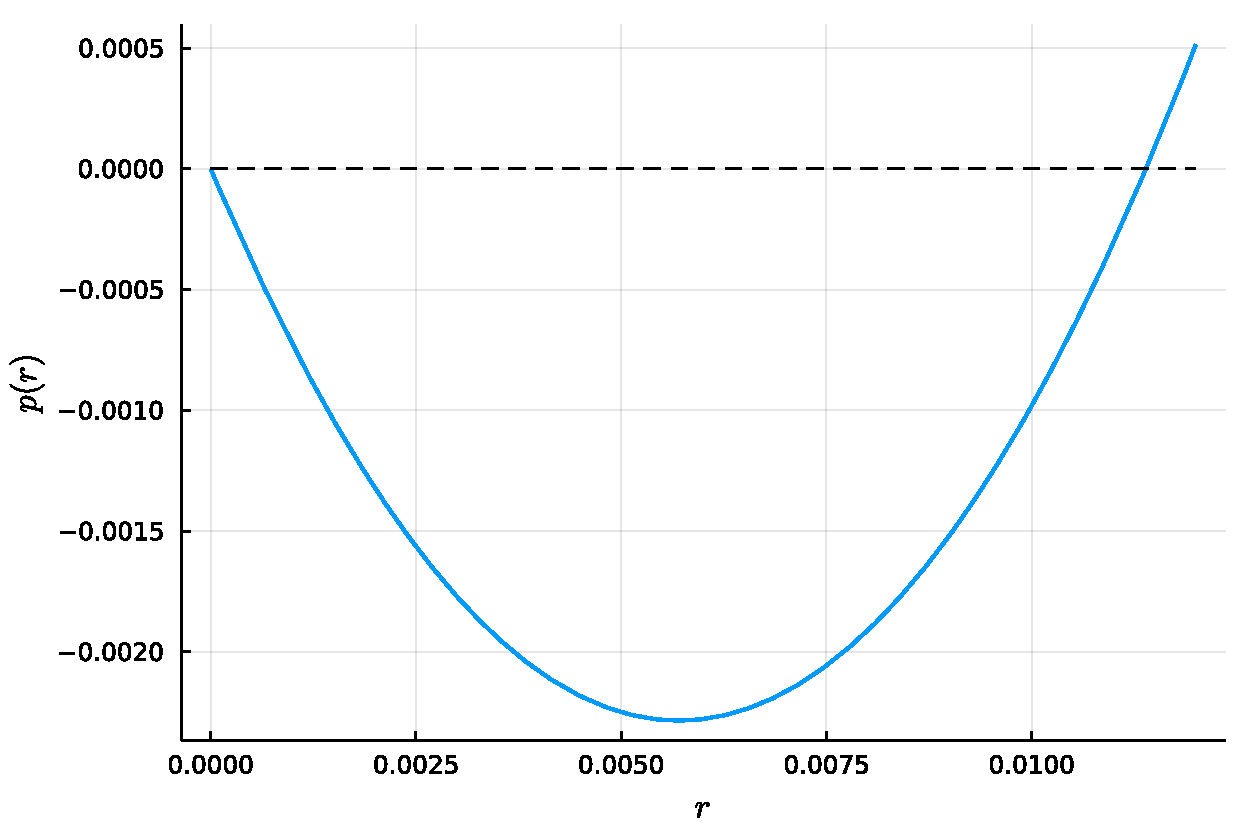
\includegraphics[keepaspectratio,scale = 0.35]{./06_VerifyPO/radii_polynomial.pdf}
	\caption{radii polynomial の概形}
\end{figure}

このことから、フーリエスペクトル法とNewton法の反復によって得た近似解の近傍 $\overline{B(\bar{\bx},r)}$ 内に $F(\bar{\bx}) = 0$ となる $\bar{\bx}$ が一意存在し、この$\bar{\bx}$ は、van der Pol方程式の周期解となる。

%\end{document}